\documentclass{article}
\usepackage[preprint,nonatbib]{neurips_2026}
\usepackage[T1]{fontenc}
\usepackage[utf8]{inputenc}
\usepackage{graphicx,booktabs,amsmath,amssymb,array}
\usepackage[hidelinks]{hyperref}
\renewcommand{\ttdefault}{pcr}
\hypersetup{pdfauthor={Idrees Aziz},pdftitle={Predicting Unfamiliar Solvers with Cross-Fitted Probability Pooling}}
\title{Predicting Unfamiliar Solvers\\with Cross-Fitted Probability Pooling}
\author{Idrees Aziz\\\href{mailto:idrees.mustafa.aziz@gmail.com}{\texttt{idrees.mustafa.aziz@gmail.com}}}
\setlength{\textfloatsep}{13pt plus 2pt minus 2pt}
\renewcommand{\arraystretch}{1.16}
\begin{document}\maketitle
\begin{abstract}
How much can a few answers reveal about an unfamiliar AI solver? We start with a model of historical evaluation results, then update its predictions using answers from the solver and its peers. Our method pools question-level evidence, corrects for solver differences, and combines two updates according to held-out probability error. In a matched local benchmark-cold evaluation with ten solvers supplying evidence, it reaches Brier ALC 0.151. A separate oracle experiment compresses questions' historical solver outcomes into four informative coordinates. Recovering those coordinates for new questions remains an open problem.
\end{abstract}

\section{A few answers, two kinds of evidence}
Two solvers can have the same accuracy while answering different questions correctly. Two questions can have the same difficulty while separating different solvers. An individual-response prediction needs more than either average.

\begin{figure}[ht]\centering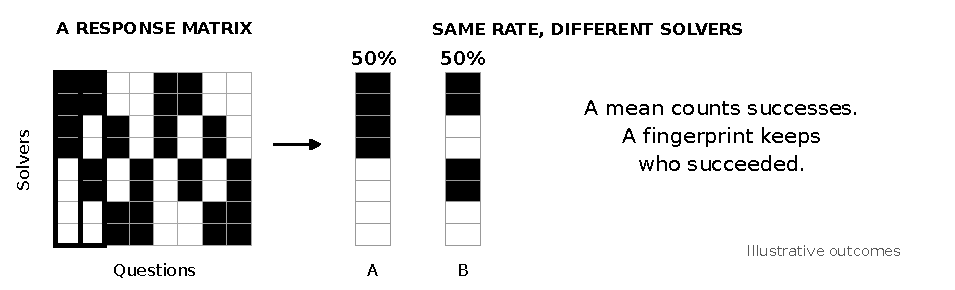
\includegraphics[width=\linewidth]{fingerprints.pdf}
\caption{A fingerprint records \emph{which} solvers succeed. The two highlighted columns have the same mean, but disagree about individual solvers. Rows are solver profiles; columns are question fingerprints. Outcomes are illustrative, with black indicating success.}
\label{fig:fingerprints}\end{figure}

The AIMS competition~\cite{aims} supplies a solver's configuration, question attributes and a limited set of revealed answers from an unfamiliar benchmark. The program predicts a success probability without running the target solver.

An answer says something about the solver, but also about the question. When other solvers have answered that question, their results supply evidence too. Our submitted method combines these signals. A separate oracle experiment asks how much of a question's behavioural fingerprint fits into four coordinates.

\clearpage
\section{The submitted method: probability pooling}
\begin{figure}[ht]\centering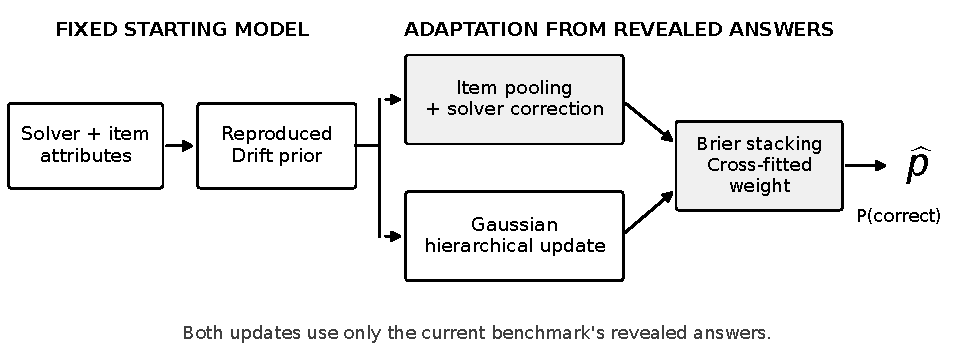
\includegraphics[width=\linewidth]{architecture.pdf}
\caption{The deployed architecture. The reproduced prior stays fixed. Revealed answers feed two adaptation rules, and a weight selected on held-out support answers combines their probabilities. Shaded boxes identify our pooling and combination layer; arrows describe the prediction flow.}
\label{fig:architecture}\end{figure}

\subsection{A starting probability}
The starting point is Team Drift's released logistic prior~\cite{drift}. Solver metadata and question attributes enter an additive model,
\begin{equation}
p^0_{si}=\sigma\!\left(b+\mathbf w_s^\top\phi(s)+\mathbf w_i^\top\psi(i)\right).
\end{equation}
Here $s$ denotes a solver configuration and $i$ a question. Hashed features describe model names, harnesses, reasoning effort, text and tool metadata. The fitted model supplies an initial probability from the attributes already present in the input.

We reproduce the released feature functions and fit the same regularized objective to 167 permitted public sources. A disk-backed implementation avoids holding the complete feature matrix in memory. Exact feature settings, data provenance and reproduction checks appear in Appendix~\ref{app:details}.

\subsection{Learn about the question and the solver}
Suppose several solvers have attempted question $i$. Let $k_i$ be their revealed successes and $n_i$ their revealed trials. A benchmark-wide log-odds correction first adjusts the prior toward the evidence on this new benchmark. Call the resulting probability for solver $s$ on item $i$ $m_{si}$. We pool it with the observed question outcomes:
\begin{equation}
\widetilde p_{si}=\frac{\kappa m_{si}+k_i}{\kappa+n_i},\qquad\kappa=0.25.
\label{eq:pool-main}
\end{equation}
This is a weighted average of a starting probability and an observed success rate. The small prior weight allows even a few answers to change a mistaken prediction. The expression follows the Beta-binomial predictive mean~\cite{beta}. Solver-specific corrections account for differences between the solvers whose outcomes enter the pool.

The new solver also receives its own regularized log-odds correction. That correction can move it above or below the pooled probabilities. Thus the method learns about a question from available solvers, then learns how the target solver differs. Sharing is possible only when the supplied evidence actually includes other solvers; a one-solver episode offers much less of it.

\clearpage
\subsection{Keep calibration evidence independent}
Support answers serve two purposes: fitting the update and measuring its prediction error. We separate these roles by removing each answer from the evidence used to construct its calibration base.

\begin{figure}[ht]\centering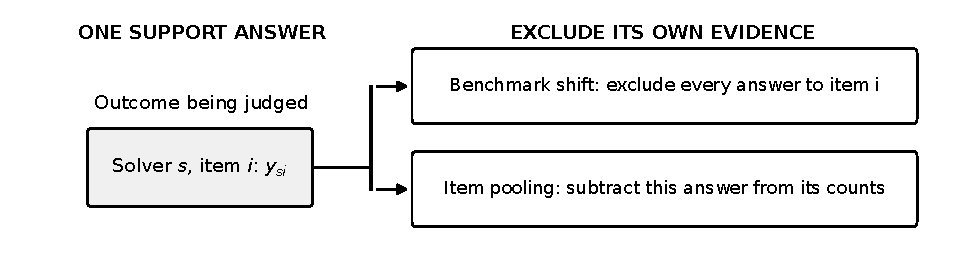
\includegraphics[width=\linewidth]{exclusion.pdf}
\caption{Two exclusions protect solver calibration. When fitting against a support answer, the benchmark shift leaves out the entire item and the pooling counts leave out that answer. These exclusions are separate from the outer cross-fitting used to select the final combination.}
\label{fig:exclusion}\end{figure}

For each support answer, we therefore remove the answer from its item counts and exclude the whole item when computing its benchmark shift. Query predictions use all currently permitted evidence. Repeated responses contribute their success and attempt counts under a shared question identity.

\subsection{Combine the updates on held-out answers}
Pooling is paired with a correlated Gaussian hierarchical update, extending the credited Drift baseline. Its benchmark, solver and question effects provide a second pattern of shrinkage. A fixed covariance shares solver offsets across the cohort.

Three folds of the revealed support answers provide predictions from both branches. Each fold refits both updates without its held labels. Write $a_t$ for the Gaussian prediction, $b_t$ for pooling, and $d_t=b_t-a_t$. The selected weight and final prediction are
\begin{equation}
w=\operatorname{clip}\!\left(\frac{\sum_t d_t(y_t-a_t)+1}{\sum_t d_t^2+1},0,1\right),
\qquad \widehat p=(1-w)a+wb.
\end{equation}
The weight minimizes held-out squared probability error, with penalty $(w-1)^2$ favouring pooling when the support set gives little reason to depart from it. This is a Brier-loss form of predictive stacking~\cite{stacking}. Weight selection uses the revealed support answers. Both branches are then fitted to the complete support set for query prediction.

\subsection{What the runtime uses}
The submitted program is CPU-only and API-free. It requires the supplied subject and item attributes, the fitted prior, NumPy and SciPy. Evidence is restricted to the current benchmark. Subject identity uses the full visible configuration; item identity includes text, attributes and tool metadata. If the benchmark identifier is missing, only unscoped evidence from the identical subject is retained.

At zero observations, the output is simply the reproduced prior, clipped away from zero and one. At later budgets, the update is recomputed from the labels supplied at that budget. Memory caches reuse fits for identical supplied evidence. Each observation budget has its own evidence set and fitted update.

\clearpage
\section{Result I: what shared evidence buys}
\subsection{Matched benchmark-cold comparison}
The core local evaluation tests BBH, GPQA, MATH and MMLU-Pro with their known source families excluded from the prior fit. A source-trained prior excludes the target benchmark and known multi-benchmark relatives. An aligned response panel supplies 192 historical configurations and 24 target configurations; the four core development cohorts contain 934, 88, 211 and 1,940 questions respectively. The 24 target configurations supply adaptation and evaluation episodes. The broad logistic prior can encounter these model identities on other permitted sources. This experiment measures transfer to held-out benchmarks with target response columns excluded from the aligned historical panel.

For each benchmark and one, three or ten sampled target solvers, we use a pool capped at approximately 1,000 solver--item pairs. Acquisition and evaluation groups are disjoint for each solver. Three fixed randomization seeds generate matched episodes, with nested budgets $n\in\{0,1,3,7,15,31\}$. Solvers may reveal answers to a question that is scored for another solver. At 31 observations, another solver has answered 29.8\% of query questions in the three-solver setting and 97.9\% in the ten-solver setting. Cohort size therefore changes both solver count and evidence coverage.

We measure squared probability error, $B_n=\operatorname{mean}(\widehat p-y)^2$. Brier ALC combines the budgets as
\begin{equation}
\mathrm{ALC}=0.1B_0+0.2B_1+0.2B_3+0.2B_7+0.2B_{15}+0.1B_{31}.
\end{equation}
Lower is better. Both adaptation methods in Table~\ref{tab:core} use the same reproduced benchmark-excluded prior and identical evidence. Only their update differs.

\begin{table}[ht]\centering
\caption{Matched local core-benchmark results. The submitted pooling settings are used throughout. Brier31 is an endpoint; ALC averages across budgets. Scores summarize the fixed local development episodes.}
\label{tab:core}
\begin{tabular}{rrrr}\toprule
Solvers & Drift update ALC & Our pooling ALC & Our pooling Brier31\\\midrule
1 & 0.2116 & 0.2106 & 0.1886\\
3 & 0.1999 & 0.1963 & 0.1627\\
10 & 0.1642 & 0.1513 & 0.0715\\
\bottomrule\end{tabular}\end{table}

With ten solvers, pooling lowers ALC by 0.0128, from 0.1642 to 0.1513, and lowers the 31-answer error from 0.0903 to 0.0715. BBH, GPQA and MMLU-Pro improve; MATH increases by 0.0011 ALC. With one solver, the ALC improvement is 0.0010 and Brier31 increases by 0.0009. Appendix~\ref{app:paired} reports the paired changes for each benchmark.

\begin{figure}[ht]\centering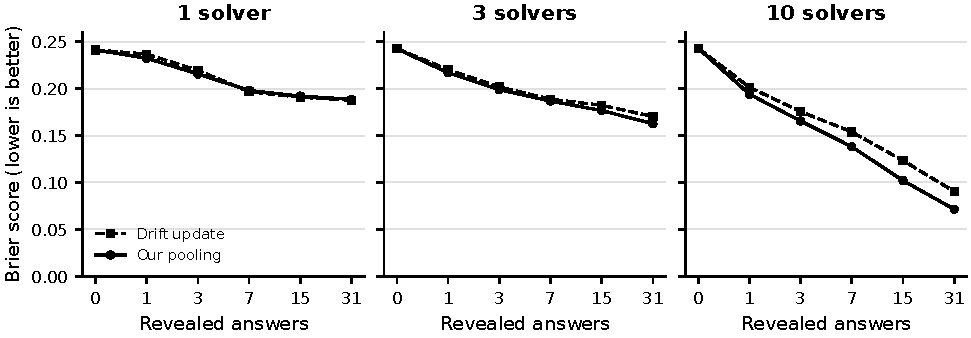
\includegraphics[width=\linewidth]{local_curves.pdf}
\caption{Matched local learning curves. Both updates receive the same prior, questions and revealed answers. Larger solver cohorts create more opportunities to share question-level evidence. Budget positions are equally spaced in $\log_2(n+1)$, as in the competition's ALC. Curves average the fixed development episodes. Paired benchmark effects appear in Appendix~\ref{app:paired}.}
\label{fig:curves}\end{figure}

\clearpage
\subsection{Beyond the favourable sharing regime}
A separate evaluation covers 43 additional public sources in 41 related-source groups. Entire groups, including related repositories and benchmark families, are excluded from the prior fit. Its 311 solver--benchmark episodes use two fixed seeds; validation groups are separate from prior-selection groups. The submitted update settings stay fixed.

Support and query texts are disjoint within each solver. Identical visible solver configurations share one budget, repeated response counts enter Brier correctly, and pairs receive equal weight. Inputs above 100,000 characters and episodes with fewer than 80 distinct texts are omitted. The analysis covers the eligible public sources under these input and sampling rules; exact-text checks operate within each source.

On this broader validation, the submitted recipe obtains ALC 0.2170 with one solver and 0.2125 with up to three. A neutral 50\% starting prior with the same update obtains 0.2153 and 0.2118. Table~\ref{tab:broad} reports the paired differences and their uncertainty. The intervals span zero in both cohorts, leaving the two starting priors unresolved by this comparison.

\begin{table}[ht]\centering
\caption{Broader held-source-group validation. $\Delta$ is neutral-prior ALC minus Drift-prior ALC; negative values favour the neutral prior. The 95\% percentile bootstrap intervals use 10,000 resamples of the 41 whole source groups, retaining paired methods, seeds and solver episodes.}
\label{tab:broad}
\small
\begin{tabular}{lrrr}\toprule
Cohort & Drift ALC & Neutral ALC & $\Delta$ ALC [95\% interval]\\\midrule
One solver & 0.2170 & 0.2153 & $-0.0016\;[-0.0050,\;0.0015]$\\
Up to three & 0.2125 & 0.2118 & $-0.0007\;[-0.0026,\;0.0011]$\\\bottomrule
\end{tabular}\end{table}

\subsection{The hosted result}
Submission \texttt{1022433} achieves hosted Brier ALC \textbf{0.190208}. Figure~\ref{fig:hosted} shows the entire formative learning curve, averaged equally over its eight solver--benchmark pairs. Its initial Brier score is 0.2779; the constant 0.5 predictor scores 0.25. At 31 observations the mean is 0.1557. The largest errors occur before the program has acquired evidence.

\begin{figure}[ht]\centering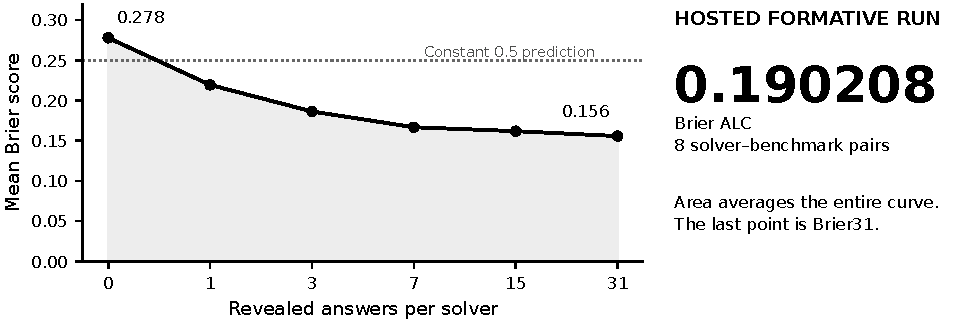
\includegraphics[width=\linewidth]{hosted_curve.pdf}
\caption{Actual hosted formative feedback. Shading marks the area summarized by ALC. Scores average eight solver--benchmark pairs equally. The hosted sample and local development bank define separate evaluations; the organizers conduct final summative scoring on a common hidden subset.}
\label{fig:hosted}\end{figure}

The matched local comparison measures the adaptation change. The hosted run measures the complete program on hidden inputs. The broad validation measures transfer across source groups. Together, these results locate the method's strength in shared question-level evidence and its main weakness in the starting probabilities.

\clearpage
\section{Result II: a four-coordinate question oracle}
Read a historical response matrix across a row and it describes a solver's behaviour. Read down a column and it describes which solvers answer a question correctly. We call this column the question's \emph{fingerprint}. Two equally difficult questions can be solved by different halves of the same solver population.

\begin{figure}[ht]\centering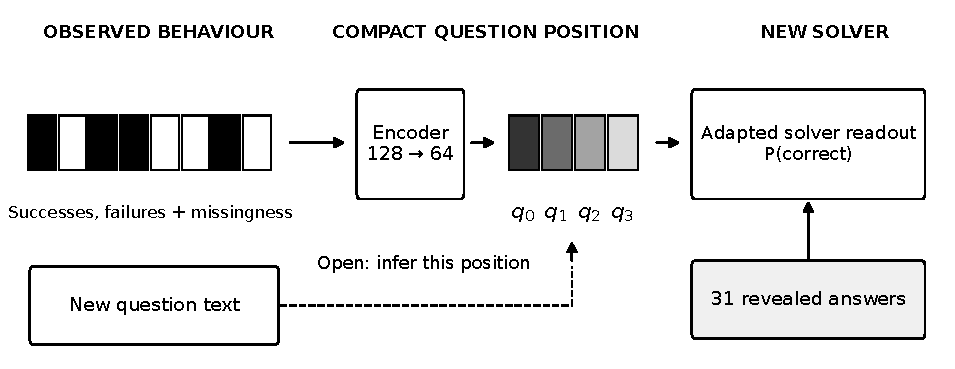
\includegraphics[width=\linewidth]{oracle.pdf}
\caption{The representation diagnostic. A behavioural fingerprint and its missingness mask enter a small encoder. Four question coordinates interact with a solver-specific readout, adapted from revealed answers. The dashed path is the open problem: predicting the same coordinates from new question text. Schematic cells illustrate the encoding and readout.}
\end{figure}

The oracle diagnostic encodes observed fingerprints and their missingness masks through a feedforward network with hidden widths 128 and 64, GELU activations and a four-number output. Training averages expected binary Brier across the observed cells of each question, then averages the question-level losses. The representation fit sees 70,952 core and 361,141 auxiliary question rows, preserving solver identities and masking unavailable responses. Its readout is
\begin{equation}
P(Y_{si}=1)=\sigma\!\left(q_{i0}+a_s+\sum_{d=1}^{3}q_{id}v_{sd}\right).
\end{equation}
The first question coordinate acts as an offset, while the other three interact with solver traits. For an excluded target solver, a source-fitted Gaussian prior over its intercept and traits is adapted through sequential Laplace updates using 31 mixed-benchmark revealed responses. Historical answers supply the evaluated question coordinates. The experiment measures prediction with these privileged behavioural positions; a deployable text encoder must recover them for new questions.

The evaluation uses 3,241 development questions from BBH, GPQA, MATH, MMLU-Pro and MuSR, with 192 historical and 24 excluded target configurations. Source calibration of the readout prior and coordinate rotations uses 12,144 questions. Ten fixed support trajectories reveal six questions per benchmark plus one rotating extra question; support groups are excluded from evaluation. Source-fitted whitening and rotations permit lower-dimensional ablations. Each readout is adapted and scored under this mixed-benchmark protocol, which differs from the benchmark-cold comparison in Table~\ref{tab:core}.

\clearpage
\subsection{How small can a useful fingerprint be?}
\begin{figure}[ht]\centering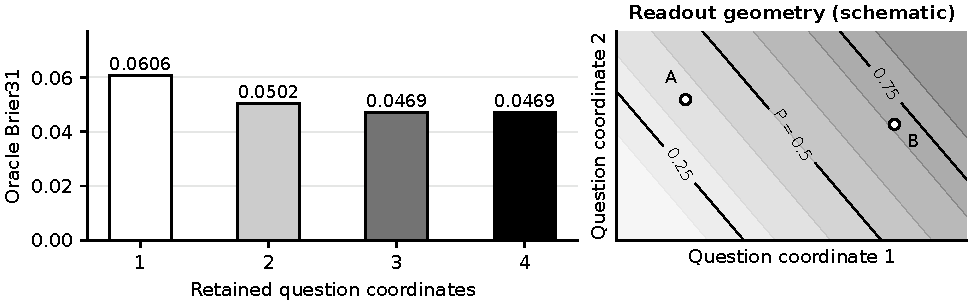
\includegraphics[width=\linewidth]{oracle_results.pdf}
\caption{Left: Brier31 after 31 revealed answers under the mixed-benchmark oracle protocol, with historical answers supplying question positions. Right: a schematic two-coordinate slice of a logistic readout. Contours show one solver's success probability; A and B mark illustrative positions.}
\label{fig:oracle-results}\end{figure}

One retained direction reaches Brier31 0.06060. Two reach 0.05023, and three reach 0.04692. All four give 0.04693. The three- and four-coordinate readouts reach essentially the same error. Source calibration constructs the retained lower-dimensional directions.

These positions preserve distinctions between the solvers that succeed on each question. A question encoder trained for this task must recover that behavioural geometry from the supplied input. The oracle provides a compact prediction target: three calibrated directions retain almost all of the four-coordinate readout's accuracy in this development cohort.

\section{Scope, attribution and reproducibility}
The submitted contribution is the cross-fitted pooling and Brier-stacking layer over a reproduced public prior. Team Drift's original feature functions, prior model and hierarchical adaptation are credited and their MIT license is retained~\cite{drift}. Performance is measured empirically through Brier error. The four-coordinate experiment evaluates a separate behavioural representation.

Training uses permitted public Measurement Data Bank outcomes, with separate benchmark-excluded fits for local validation. The exact submitted archive passes the organizer's checker and isolated reference-parity tests. It runs without APIs, downloads or a GPU. Appendix~\ref{app:details} records data revisions, exclusions, implementation checks and reproduction requirements. OpenAI Codex assisted implementation, analysis and writing.

The two results meet at the same question: what can an answer tell us beyond its own cell in the response matrix? The submitted update transfers evidence through shared questions. The oracle transfers it through a compact behavioural representation. Recovering that representation for unseen questions remains the missing connection.

\clearpage
\begin{thebibliography}{9}\raggedright\urlstyle{same}
\bibitem{aims} AIMS. The Predictive AI Evaluation Competition at NeurIPS 2026. Rules, interface and evaluation protocol.\newline\url{https://aims.stanford.edu/competition/}.
\bibitem{drift} Alex Alvord / Cloud Lab Works LLC. Team Drift: AIMS / NeurIPS 2026 PAIEC. Released implementation and training recipe, commit \texttt{5a67dfcbaf8742f639edbfb96f15ee6efe3eed04}.\newline\url{https://github.com/cloudlabworks/aims-team-drift}.
\bibitem{db} AIMS Foundations. The AI Measurement Data Bank. Public tables and benchmark-level provenance.\newline\url{https://huggingface.co/datasets/aims-foundations/measurement-db}.
\bibitem{beta} Bob Carpenter. Getting Started with Bayesian Statistics. Bernoulli inference and Beta conjugacy.\newline\url{https://bob-carpenter.github.io/stan-getting-started/stan-getting-started.html}.
\bibitem{stacking} Yuling Yao, Aki Vehtari, Daniel Simpson, and Andrew Gelman. Using stacking to average Bayesian predictive distributions (with discussion). \emph{Bayesian Analysis}, 13(3):917--1007, 2018.\newline\url{https://doi.org/10.1214/17-BA1091}.
\end{thebibliography}

\clearpage
\appendix
\section{Exact statistical specification}\label{app:details}
\subsection{The cross-benchmark starting point}
We reproduce Team Drift's released logistic prior~\cite{drift}, retaining its feature functions and training settings. For solver $s$ and item $i$,
\begin{equation}
p^0_{si}=\sigma\!\left(b+\mathbf w_s^\top\phi(s)+\mathbf w_i^\top\psi(i)\right),\qquad \sigma(z)=\frac{1}{1+e^{-z}}.
\end{equation}
The subject features hash the model name, provider, harness, reasoning effort, dates and configuration fields at several granularities. Item features hash words, word pairs, length bins, supplied attributes and tool metadata. Text features receive source-fitted inverse-document-frequency weights and row normalization. Inference evaluates the additive probability model on the supplied attributes.

The deployment prior is fitted to 167 public binary benchmark sources at the pinned AI Measurement Data Bank revision~\cite{db}. It retains at most 10,000 observed items per source, using the released deterministic selection. Repeated trials become success and attempt counts for each solver--item pair. If source $b$ has $N_b$ attempts, each likelihood term has weight $N_b^{-1/2}$. Subject and item ridge coefficients are both 0.01. Our disk-backed fitter evaluates the same objective without loading the complete feature matrix into RAM. The IDF array matches the historical release hash. The fitted weights come from our reproduction of the training objective.

\subsection{Let the evidence override a mistaken prior}
The prior can be wrong about an unfamiliar benchmark. The adaptation rule corrects that error using revealed outcomes. Cross-fitting separates each solver's calibration target from the evidence used to construct its starting probability.

For each item $i$ currently observed, let $n_i$ be the number of revealed trials and $k_i$ their successes, pooled over permitted solvers. Define the shared item prior $\bar p_i$ as the mean of $p^0_{si}$ over the current solver cohort. A regularized log-odds shift $g$ calibrates these shared priors using one fractional outcome $k_i/n_i$ per distinct observed item. This prevents a frequently observed item from dominating the benchmark shift solely through its multiplicity.

The shift minimizes logistic cross-entropy plus four soft prior observations centred on zero shift. For offsets $z_i=\operatorname{logit}\bar p_i$, $\mu=\operatorname{mean}_i\sigma(z_i)$ and $a=\operatorname{logit}\mu$, its objective is
\begin{equation}
L(g)=\sum_i\left[\operatorname{softplus}(z_i+g)-\frac{k_i}{n_i}(z_i+g)\right]
+4\left[\operatorname{softplus}(a+g)-\mu(a+g)\right].
\end{equation}
For an observed item, its calibration shift $g_{-i}$ is fitted using the other items only; a previously unobserved query uses the all-support shift. We then use the target solver's own prior,
\begin{equation}
m_{si}=\sigma\!\left(\operatorname{logit}p^0_{si}+g_{-i}\right),\qquad
\widetilde p_{si}=\frac{\kappa m_{si}+k_i}{\kappa+n_i},\qquad\kappa=0.25.
\label{eq:pool}
\end{equation}
Equation~\ref{eq:pool} has the form of a Beta-binomial predictive mean~\cite{beta}. We use the conjugate expression as a regularized predictive pooling rule and estimate solver differences through log-odds corrections. A small $\kappa$ lets observed outcomes override the starting probability.

Each solver also receives a regularized log-odds correction, fitted with ridge precision 16. For a support answer $y_{si}$, its calibration base removes that answer from the counts:
\begin{equation}
\widetilde p^{\,\mathrm{support}}_{si}
=\frac{\kappa m_{si}+k_i-y_{si}}{\kappa+n_i-1}.
\end{equation}
The benchmark shift for that base excludes the whole item. Removing both paths matters: otherwise the label used to judge the solver has already moved its supposed prior in the same direction. Query predictions use all evidence permitted at the current budget. Repeated trials retain their success and attempt counts within each question identity.

\subsection{Choose the combination for Brier error}
The pooling prediction is combined with a correlated Gaussian hierarchical correction of the prior. The latter extends Drift's benchmark, solver and item log-odds update: benchmark and item standard deviations are 1.5, solver standard deviation is 0.8, and the fixed solver correlation matrix is $0.1I+0.9\mathbf1\mathbf1^\top$. This covariance imposes common shrinkage across solver offsets.

Three folds of the currently revealed answers generate held-out predictions from both updates. Let $a_t$ be the Gaussian prediction, $b_t$ the pooling prediction and $d_t=b_t-a_t$. The weight on pooling is
\begin{equation}
w=\operatorname{clip}\!\left(\frac{\sum_t d_t(y_t-a_t)+1}{\sum_t d_t^2+1},0,1\right),\qquad
\widehat p=(1-w)a+wb.
\end{equation}
This minimizes held-out Brier error with penalty $(w-1)^2$; the penalty favours pooling when little support evidence distinguishes the updates. Each fold refits both methods without its held labels. The held-out support predictions determine the weight. The procedure adapts predictive stacking~\cite{stacking} to squared probability error.




\section{Data provenance and implementation checks}
All training outcomes come from permitted public Measurement Data Bank sources at revision \texttt{54074453da7b9911be0f48e4c560be547bc84d21}. The deployment prior uses 624,900 selected source-item records and 12,839,906 aggregated solver--item rows. Local comparisons use separately fitted priors with the target source groups excluded. Duplicate checks cover exact question text within the episode sources. The remaining generalization questions concern semantic duplicates across repositories, further benchmark families and future solver populations. The local bank and related solver configurations have been inspected during development.

The exact submitted ZIP contains the trained prior, NumPy/SciPy adaptation and the official \texttt{predict(input,labeled)} entry point. It needs no API key, network inference, model download or GPU. The organizer's ZIP checker passes. An isolated exact-archive test verifies 168 dispatch predictions against the reference adaptation to within $6\times10^{-17}$, including unequal support sizes, repeated trials, tool-distinct items, unseen target subjects and benchmark isolation. The disk-backed trainer reproduces the unchanged upstream trainer on a fixture; real-data preprocessing agrees exactly on three checked sources. OpenAI Codex assisted implementation, analysis and writing.


\clearpage
\section{Reproduction map}
The source manifest records all 167 benchmark names, the pinned dataset revision and fitted-artifact hashes. \path{scripts/reproduce_drift_prior_v80.py} reconstructs the prior from the public tables with disk-backed sparse features. \path{scripts/evaluate_drift_prior_v80.py} produces Table~\ref{tab:core}; \path{scripts/broad_prior_audit_v81.py} defines the source-group splits and broader comparison, and \path{scripts/verify_broad_prior_audit_v81.py} independently checks selection, aggregation, split boundaries and paired source-group bootstrap calculations. The measured oracle figure is read directly from the coordinate-ablation result generated by \path{scripts/coordinate_brier_ablation_v42.py}.

\path{models/drift_pooling_runtime_v82.py} implements the submitted dispatch and \path{models/subject_adaptation_v79.py} implements the subject-specific pooling layer. \path{scripts/package_drift_pooling_v82.py} builds the explicit-allowlist scoring ZIP, and \path{scripts/check_drift_pooling_zip_v82.py} tests that exact archive in a fresh process with network access blocked. The archive SHA-256 is
\begin{quote}\small\ttfamily
b0aef886620c7ba3545ab7b132336b969079\\
ee5160d758d67125703b51a9ffd1.
\end{quote}
Local probability pooling clips its numerical bases away from zero and one. The zero-answer prediction is the starting prior, clipped to $[0.001,0.999]$. Acquired labels are filtered to the same anonymous benchmark identifier; if that identifier is missing, only unscoped evidence from the identical subject is retained. Item identity includes content, supplied features and tool metadata. The runtime refits support evidence when its signature changes and reuses cached fits for identical evidence.

Code, fitted weights, development records and report sources are available at \url{https://github.com/idreesaziz/aims-solver-profiles}. The repository includes the credential-free scoring archive, a portable prior trainer and scripts that reproduce the tables and confidence intervals. Raw Measurement Data Bank tables retain their source access terms and licenses.

\subsection{Run the fitted predictor without training}
Python 3.12.10, NumPy 2.2.4 and SciPy 1.15.2 were used for the local archive checks. The fitted archive contains its payload and requires no raw dataset to run inference. After extracting it into a directory named \texttt{submission}, a minimal smoke test is:
\begin{verbatim}
python -m pip install numpy==2.2.4 scipy==1.15.2
cd submission
python -c "import model; print(model.predict([
{'normalized_name':'example','harness':'example'},
{'item_content':'What is 2+2?','benchmark_id':'demo'}], []))"
\end{verbatim}
The command checks loading and dispatch by returning a finite probability in $[0,1]$. In the development checkout, run \path{scripts/check_drift_pooling_zip_v82.py} against the exact archive for the stronger isolation and reference-parity checks described above. The organizer's \path{check_submission_zip.py} provides the interface check.

\subsection{Rebuild the experiments}
The deployment prior uses all 167 source names in the pinned upstream \path{report/TRAINING_SOURCES.json}. Reproduction uses this exact revision and source list. The disk-backed fitter downloads missing permitted public tables through Hugging Face, subject to dataset access and source terms. Its \texttt{DATA} and \texttt{OUT} paths identify the local data and feature-cache roots and must be set for another machine. Local core validation requires the benchmark-excluded prior. The full fitted payload supplies deployment predictions.

The archived local evaluation scripts depend on the aligned response panel, grouped split manifests and frozen prediction caches. The repository supplies the oracle's fitted numerical arrays, scoring plans and episode-level results. Its reproduction guide identifies the additional data-preparation inputs needed to rerun representation training. Inference, prior fitting and statistical aggregation have separate runnable entry points.


\clearpage
\section{Paired effects and statistical uncertainty}\label{app:paired}
The local comparison uses the same solver, question partition, seed and revealed answers for both updates. Subtracting their episode ALCs removes variation shared by the two methods. Table~\ref{tab:paired} averages these paired differences within each benchmark. Each core benchmark contributes equally to the reported mean.

\begin{table}[ht]\centering
\caption{Our pooling ALC minus Drift-update ALC on each core benchmark. Negative values favour pooling. Values average the three matched randomization seeds and sampled target configurations.}
\label{tab:paired}
\begin{tabular}{lrrr}\toprule
Benchmark & One solver & Three solvers & Ten solvers\\\midrule
BBH & $-0.0067$ & $-0.0099$ & $-0.0173$\\
GPQA & $-0.0034$ & $-0.0048$ & $-0.0146$\\
MATH & $+0.0132$ & $+0.0073$ & $+0.0011$\\
MMLU-Pro & $-0.0074$ & $-0.0067$ & $-0.0204$\\
\bottomrule\end{tabular}\end{table}

The four core benchmarks define a small, curated comparison. Reporting their separate effects makes the MATH reversal and the gains on the other three benchmarks visible. The shared-item coverage increases with cohort size, so the ten-solver comparison measures both richer solver evidence and denser question overlap.

For the broader comparison, the resampling unit is a related-source group. We draw 41 groups with replacement, retain all their solver episodes and seeds, and recompute the paired mean ALC difference using the original pair weights. The 2.5th and 97.5th percentiles of 10,000 draws form the intervals in Table~\ref{tab:broad}. The script \path{scripts/analyze_recent_runs_v86.py} computes these intervals with NumPy seed 860. This block resampling preserves dependence among sources from the same repository or family, repeated seeds and solver configurations within a source. Cross-group dependencies remain a limitation of the interval calculation.

The broad one-solver comparison contains 86 pair episodes; the up-to-three comparison contains 225. Prior selection used separate source groups and was frozen before validation. The intervals describe uncertainty in this public development comparison. Broader populations of benchmarks and solvers require further evaluation.

The hosted result averages the eight solver--benchmark pairs in the organizer's formative sample. Its six budget scores describe one sampled evaluation. The oracle averages ten fixed adaptation trajectories for 24 target configurations on the fixed mixed-benchmark bank. Each result is reported with its own evaluation unit and protocol.

\end{document}

